%\section{}
\clearpage
\section{Marco teórico}
    La Asociación de Internet MX (AIMX) es una asociación civil mexicana que tiene a los principales actores de la industria 
    de internet como socios y aliados. Provee información sobre distintas temáticas alrededor del mundo digital y se aun ubicado 
    en un marco de referencia en temas claves para el desarrollo e implementación de proyectos normativos y de política pública 
    que coadyuven en la productividad y la competitividad de México.\\ 

    En su último  estudio titulado ``Estudio de Búsqueda de Empleo por Internet en México 2021'', expuso que más de la mitad de 
    los candidatos buscan trabajo en bolsas de trabajo en línea o redes sociales ya que en los ultimos dos años
    la pandemia a causa del COVID beneficio la busqueda digital de trabajo.\\
    \newline
    La transformación digital y la necesidad de inmediatez ha impulsado de manera significativa el uso de los smartphones con 
    en la búsqueda de trabajo en línea, más del 60\% de los mexicanos busca trabajo por internet de una muestra de 10,864 personas, 
    el 59\% hombres y 41\% mujeres de entre 25 a 39 años, de los cuales, la mayoría de los que buscan empleo estan en el rango de 
    edad de 25 a 39 años y predominan las personas con estudios nivel Licenciatira.
    Cabe resaltar que solo el 43\% de dicha muestra no tiene trabajo. (Ver figura \ref{mark:pob}) 
    \begin{figure}[H]
        \begin{center}
            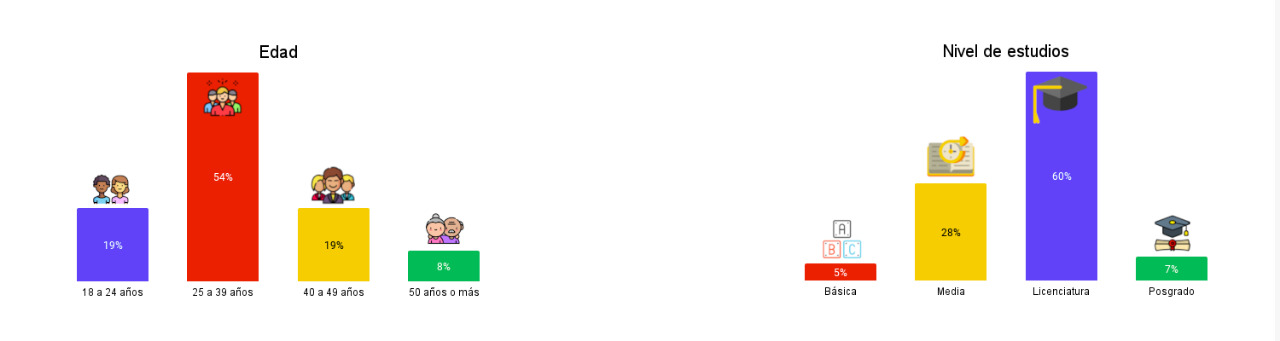
\includegraphics[width=.9\textwidth]{antecedentes/imagenes/porcen.jpeg}
        \end{center}
        \caption{Población que busca trabajo en linea.}
        \label{mark:pob}
    \end{figure}
    


    Las herramientas utilizadas con base en sus muestras se tiene que el 66\% de las personas que buscan empleo o una mejor 
    oportunidad laboral tiene instalada un app de bolsa de trabajo y el 55\% revisó vacantes en sus redes sociales y a pesar de esto aun se mantiene a la cabeza el uso de una bolsa de
    trabajo en internet con el 70\% un factor que ya vieron las empresas, ya que el 87\% de ellas busca
    talento a través de estas plataformas , seis de cada 10 candidatos obtienen entrevistas gracias a ellas. (Ver figura \ref{mark:med})

    \begin{figure}[H]
        \begin{center}
            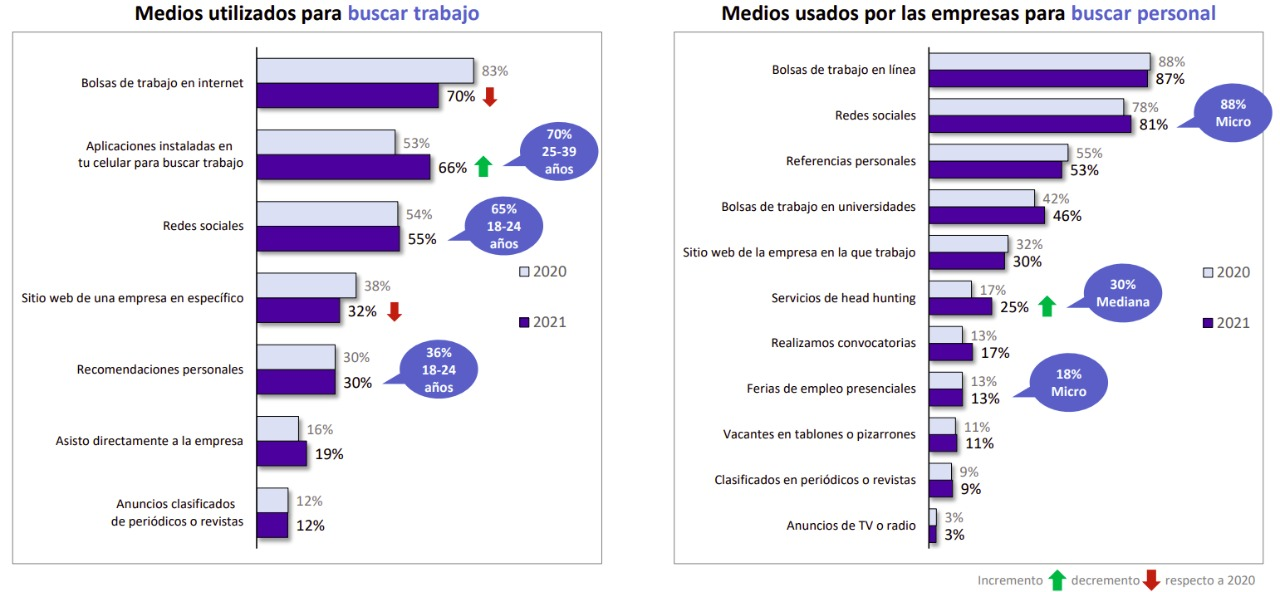
\includegraphics[width=.7\textwidth]{antecedentes/imagenes/medios.jpeg}
        \end{center}
        \caption{Medios para buscar trabajo y buscar personal AIMX 2021.}
        \label{mark:med}
    \end{figure}


    Gracias al uso de estas plataformas ha mejorado el tiempo en que un reclutador tarda en contactar a los candidatos, el principal
    medio es por llamada y continúa creciendo el uso de WhatsApp. Los beneficios económicos son más relevantes al evaluar una oferta de
    trabajo, en tanto que los reclutadores se basan más en la experiencia laboral y conocimientos. (Ver figura \ref{mark:fac})

    \begin{figure}[H]
        \begin{center}
            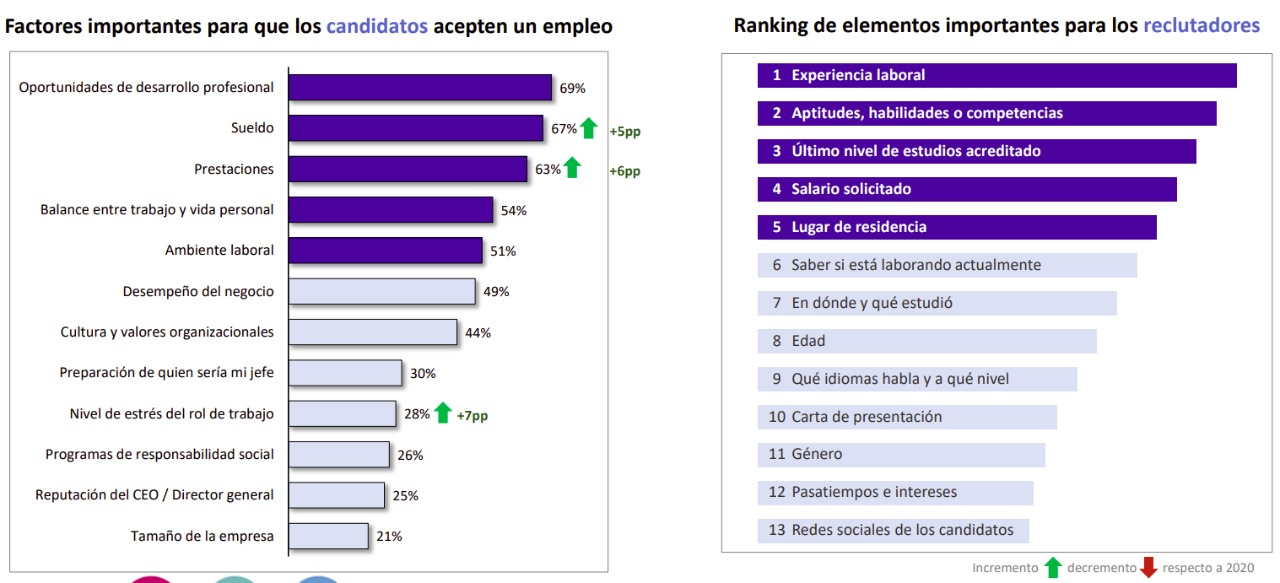
\includegraphics[width=.7\textwidth]{antecedentes/imagenes/consideraciones.jpeg}
        \end{center}
        \caption{Factores para buscar emplo y contatar personal AIMX 2021.}
        \label{mark:fac}
    \end{figure}


    Por otro lado, el seguimiento y la facilidad de postularse son los principales aspectos que buscan los candidatos en las bolsas 
    de trabajo, aunque toma relevancia que éstas cuenten con una app, mientras que los reclutadores buscan mayormente que las bolsas 
    de trabajo sean efectivas, aunque se vuelven relevantes los aspectos relacionados a usabilidad y funciones. (Ver figura \ref{mark:efi})
    \begin{figure}[H]
        \begin{center}
            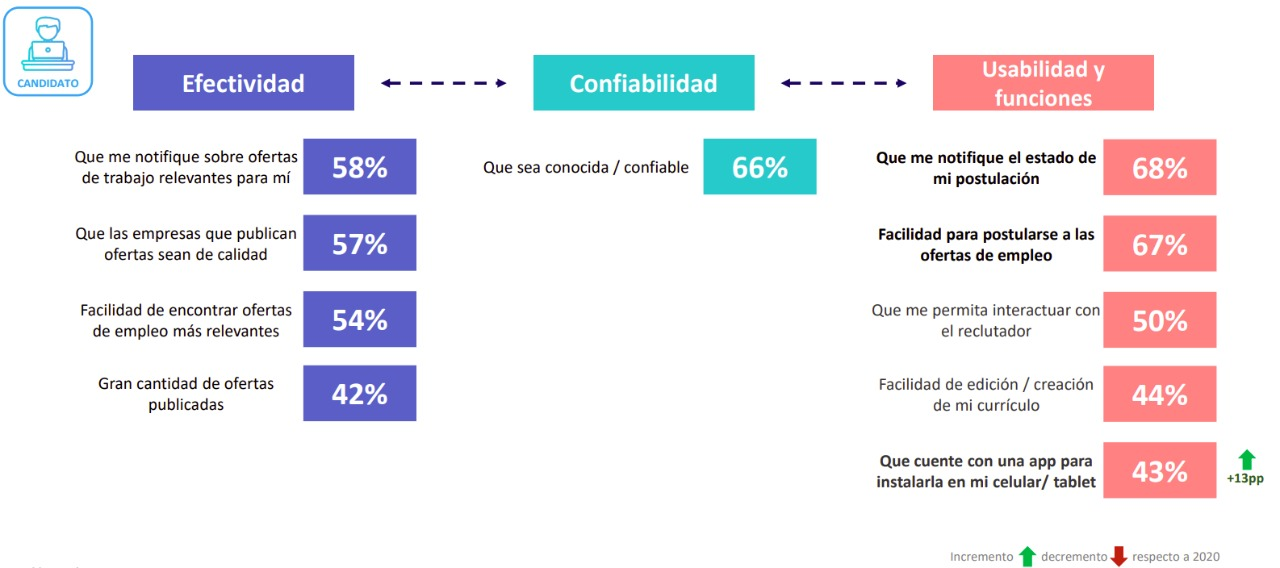
\includegraphics[width=.6\textwidth]{antecedentes/imagenes/prefC.jpeg}
            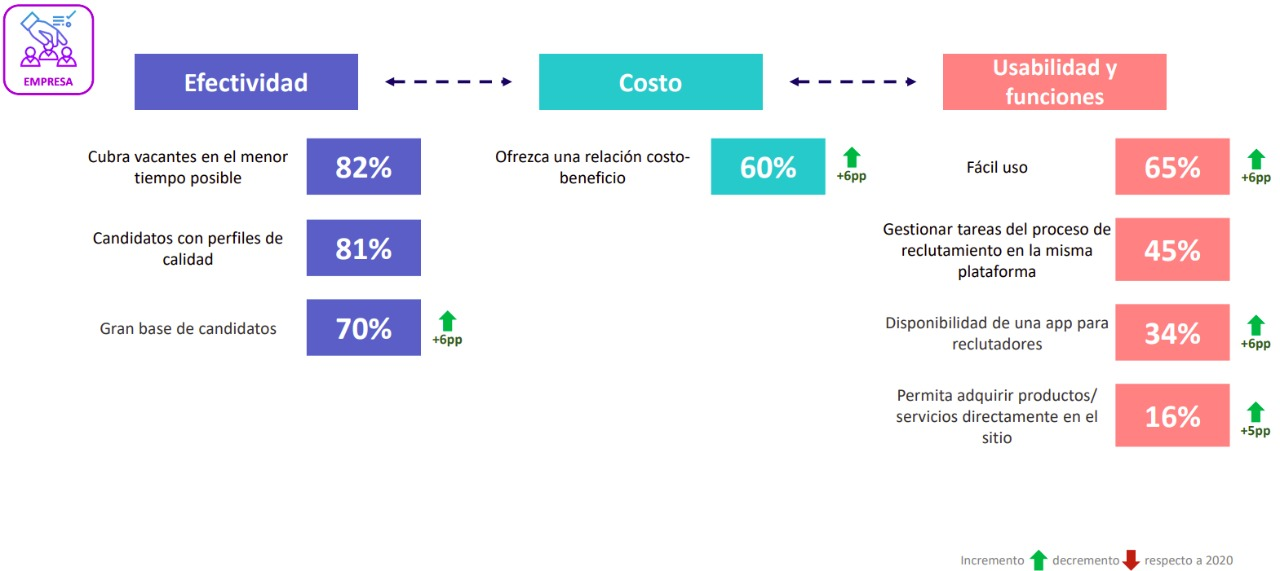
\includegraphics[width=.6\textwidth]{antecedentes/imagenes/prefE.jpeg}
        \end{center}
        \caption{Eficiencia de la plataforma para ambos usuarios.}
        \label{mark:efi}
    \end{figure}

    La principal bolsa de trabajo  de los candidatos y las empresas es OCCMundial, mientras de los candidatos recurren tambien a las 
bolsas de empleo más populares como Computrabajo, Indeed y LinkedIn los reclutadores además usan las redes sociales para buscar talento, la
figura \ref{mark:med} muestra la preferencia de plataformas por candidatos y reclutadores en el 2021.
\begin{figure}[H]
    \begin{center}
        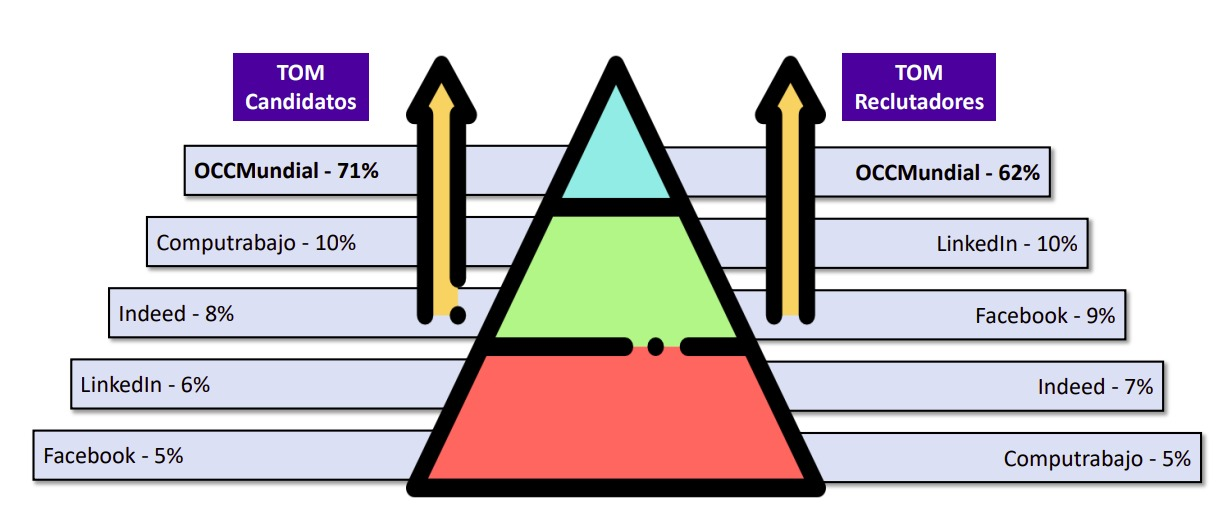
\includegraphics[width=.7\textwidth]{antecedentes/imagenes/topbdt.jpeg}
    \end{center}
    \caption{Bolsas de trabajo más populares.}
    \label{mark:med}
\end{figure}


Cabe mencionar que los propios candidatos recomiendan las siguientes bolsas de trabajo:
\begin{itemize}
    \item Jobomas
    \item Empleo.gob.mx 
    \item Talenteca Bumeran
\end{itemize}



    
